\documentclass[12pt, a4paper]{article}
\usepackage{import}
\usepackage{QuatumPreamble}

\title{Equivalent Circuits}
\date{\(10^\mathrm{{th}}\) November 2022}
\author{Lee Farrugia}

\begin{document}

\maketitle
\thispagestyle{titlepagestyle}
\pagestyle{mystyle}

\section*{Abstract}
This experiment was conducted in order to investigate the electromagnetically induced system, specifically the lambda system. It indicated that the transition between state 1 and state 2 is forbidden, thus they are referred to as transparent. From the experiment conducted, the Hamiltonian matrix obtained is concurrent with the observed literature, however the density matrix obtained was incorrect. Therefore, the results obtained were inherently wrong.

\section{Introduction \& Theoretical Background}
Electromagnetically induced transparency was fist theorized by Harris et al in 1990. This occurs when using a strong laser field is used to drive the system, while the probe field reduces and eliminates some of the transitions~\parencite{ijazEIT}.

This experiment was conducted in order to compute and understand what is referred to as a Lambda system and the electromagnetically-induced transparency (EIT). The Lambda system is a system in Atomic Physics when an atom/s inside a gas can transition only between specific levels which from the greek letter \(\mathrm{\Lambda}\). The transitions allowed are between \(1 \leftrightarrow 3\) and \(2 \leftrightarrow 3\), while eliminating the \(1 \leftrightarrow 2\) transition by making it stop absorbing light from a probe field. This results that many of the atoms in the gas become transparent hence EIT\,. These transitions can be seen in figure~\ref{fig:Transition_Diagram}.

\begin{figure}[H]
  \centering
  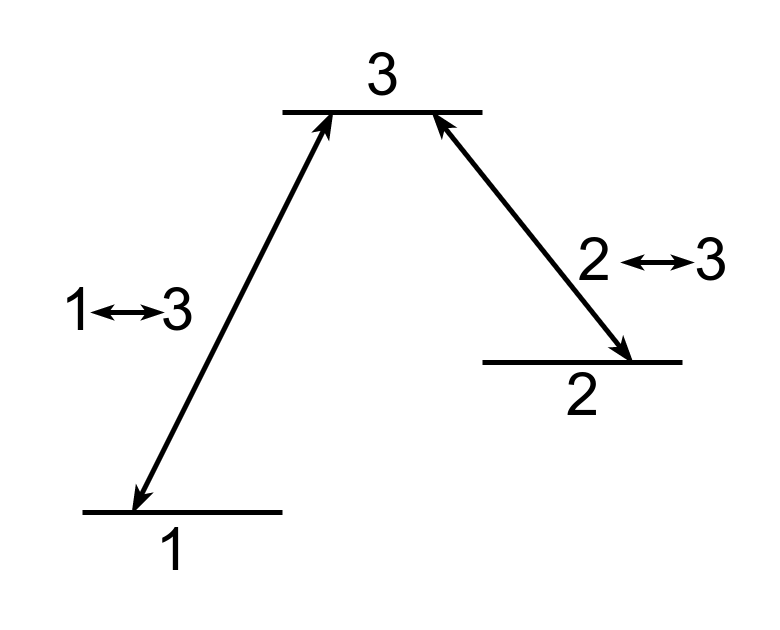
\includegraphics[width=0.4\textwidth]{Transition Diagram.png}\caption{Diagram of the transitions in the lambda system}\label{fig:Transition_Diagram}
\end{figure}

\section{Materials \& Methods}
  \subsection{Language and Packages}
    Python 3.10.6, Numpy, Scipy, Matplotlib.pyplot\,.

  \subsection{Methodology}
  \begin{enumerate}
    \item In order to simulate the system and compute it, the Hamiltonian governing the system is considered, which can be written as:
    \begin{equation}
      \hat{H} = \hat{H_0} + \hat{H}_{pump} + \hat{H}_{probe}\,, 
    \end{equation}
    where 
    \begin{align}
      \hat{H_0}&=\hbar\omega_1\ket{1}\bra{1}+\hbar\omega_2 \ket{2}\bra{2} + \hbar\omega_3\ket{3}\bra{3}\,,\\
      \hat{H}_{pump} &= \hbar \varepsilon_{pump}(e^{-i\omega_{pump}t}\ket{2}\bra{3} + e^{i\omega_{pump}t}\ket{3}\bra{2})\,,\\
      \hat{H}_{probe} &= \hbar \varepsilon(e^{-i\omega_{probe}t}\ket{1}\bra{3} + e^{i\omega_{probe}t}\ket{3}\bra{1})\,. 
    \end{align}
    \(\ket{j}\) corresponds to the three different states that can be sene in figure~\ref{fig:Transition_Diagram} and their corresponding frequencies \(\omega_j\), \(\varepsilon_{pump}\) and \(\varepsilon_{probe}\) signify the strength of the pump and probe fields respectively which are a frequencies \(\omega_{pump} = \omega_(23) = \Delta_{pump}\) and \(\omega_{probe} = \omega_{13} + \Delta_{probe}\).    By setting \(\Omega_1 = \omega_1 - \Delta_{probe}\), \(\Omega_2 = \omega_3 - \Delta_{pump}\) and \(\Omega_3 = \omega_3\) the following transformation are to be done on the Hamiltonian,
    \begin{align}
      \ket{j} &\rightarrow e^{- i \Omega_j t}\ket{j}, j(=1,2,3)\,\\
      \hat{H} &\rightarrow \hat{H} - \sum_{j} \hbar \Omega_j \ket{j}\bra{j}\,.
    \end{align}
    These transformations will result in a three dimensional matrix without time dependence. Furthermore taking \(\omega_{pump} = \Omega_2 - \Omega_3\) and \(\omega_{probe} = \Omega_1 - \Omega_3\) the Hamiltonian parts would become:
    \begin{align}
      \hat{H}_{probe} &= \hbar \varepsilon_{probe}(e^{-i \Omega_3 - \Omega_1 t}\ket{1}\bra{3} + e^{i \Omega_3 - \Omega_1}\ket{3}\bra{1})\\
      &= \hbar \varepsilon_{probe}(e^{-i \Omega_1 t}\ket{1}e^{i \Omega_3 t}\ket{3} + e^{-i \Omega_3 t}\ket{1}e^{i \Omega_1 t}\ket{1})\\
      &= \hbar \varepsilon_{probe}(e^{-i \Omega_1 t}e^{i \Omega_1 t}\ket{1}\bra{3} + e^{-i \Omega_3 t}e^{i \Omega_3 t}\ket{3}\bra{1})\\
      &= \hbar \varepsilon_{probe}\ket{1}\bra{3} + \hbar \varepsilon_{probe}\ket{3}\bra{1}\\
      \hat{H}_{pump} &= \hbar \varepsilon_{probe}(e^{-i \Omega_3 - \Omega_1 t}\ket{1}\bra{3} + e^{i \Omega_3 - \Omega_1}\ket{3}\bra{1})\\
      &= \hbar \varepsilon_{probe}(e^{-i \Omega_2 t}\ket{2}e^{i \Omega_3 t}\ket{3} + e^{-i \Omega_2 t}\ket{2}e^{i \Omega_3 t}\ket{3})\\
      &= \hbar \varepsilon_{pump}(e^{-i \Omega_2 t}e^{i \Omega_2 t}\ket{2}\bra{3} + e^{-i \Omega_3 t}e^{i \Omega_3 t}\ket{3}\bra{2})\\
      &= \hbar \varepsilon_{pump}\ket{2}\bra{3} + \hbar \varepsilon_{pump}\ket{3}\bra{2}\,,\\
    \end{align}
    therefore the combined Hamiltonian becomes:
    \begin{equation}
      \begin{split}
        \hat{H} = &\hbar(\Omega_1 + \Delta_{probe}) + \hbar(\Omega_2 + \Delta_{pump}) + \hbar\Omega_3 \\ &+ \hbar \varepsilon_{probe}\ket{1}\bra{3} + \hbar \varepsilon_{probe}\ket{3}\bra{1} \\ &+ \hbar \varepsilon_{pump}\ket{2}\bra{3} + \hbar \varepsilon_{pump}\ket{3}\bra{2} \,.
      \end{split}
    \end{equation}
    Thus, the Hamiltonian matrix is:
    \begin{gather}
      \tilde{H} =
      \begin{bmatrix}
        \hbar\Delta_{probe} & 0 & \hbar\varepsilon_{probe}\ket{1}\bra{3}\\
        0 & \hbar\Delta_{pump} & \hbar \varepsilon_{pump}\ket{2}\bra{3}\\
        \hbar \varepsilon_{probe}\ket{3}\bra{1} & \hbar \varepsilon_{pump}\ket{3}\bra{2} & 0
      \end{bmatrix}
    \end{gather}
    \item The density matrix that is obtained from the Hamiltonian by first defining the rabi frequencies as:
    \begin{align}
      \Omega_{probe} &= \frac{\varepsilon_{probe}\ket{1}\bra{3}}{\hbar}\\
      \Omega_{pump} &= \frac{\varepsilon_{pump}\ket{2}\bra{3}}{\hbar}\,.
    \end{align}
    using these values and the fact that \(\rho = \sum_{n}P_n\ket{n}\bra{n}\) we obtain these following results:
    \begin{align}
      \dot{\tilde{\rho}}_{11} &= i \frac{\varepsilon_{probe}\ket{1}\bra{3}}{2\hbar}(\rho_{21}-\rho_{12}) \approx 1\\
      \dot{\tilde{\rho}}_{12} &= (-\gamma_{12} + i (\Delta_{pump}- \Delta_{probe}))\tilde{\rho}_{12} - i \frac{\varepsilon_{pump}\ket{2}\bra{3}}{2\hbar}\tilde{\rho}_{13} + i \frac{\varepsilon_{probe}\ket{1}\bra{3}}{2\hbar}\tilde{\rho}_{32}\\
      \dot{\tilde{\rho}}_{13} &= (- \gamma_{13} + i\Delta_{pump})\tilde{\rho}_{13} - i \frac{\varepsilon_{pump}\ket{2}\bra{1}}{2\hbar}(\tilde{\rho}_{32}-\tilde{\rho}_{11}) - i \frac{\varepsilon_{probe}\ket{1}\bra{3}}{2\hbar}\tilde{\rho}_{12}\\
      \dot{\tilde{\rho}}_{21} &= (-\gamma_{21}-i(\Delta_{pump}-\Delta_{probe}))\tilde{\rho}_{21}+i\frac{\varepsilon_{pump}\ket{2}\bra{3}}{2\hbar}\tilde{\rho}_{31}-i \frac{\varepsilon_{probe}\ket{1}\bra{1}}{2\hbar}\tilde{\rho}_{23}\\
      \dot{\tilde{\rho}}_{22} &= - \gamma_{2} \rho_{22} - i \frac{\varepsilon_{probe}\ket{1}\bra{3}}{2\hbar}(\rho_{21}- \rho_{12}) - i \frac{\varepsilon_{probe}\ket{2}\bra{1}}{2\hbar}(\rho_{23} - \rho_{22}) \approx 0\\
      \dot{\tilde{\rho}}_{23} &= (-\gamma_{23} - i \Delta_{pump})\tilde{\rho}_{23} + i \frac{\varepsilon_{pump}\ket{2}\bra{1}}{2\hbar}(\tilde{\rho}_{33} - \tilde{\rho}_{22}) - i \frac{\varepsilon_{probe}\ket{1}\bra{3}}{2\hbar}\tilde{\rho}_{21}\\
      \dot{\tilde{\rho}}_{31} &= (-\gamma_{31} - i \Delta_{pump})\tilde{\rho}_{31} + i \frac{\varepsilon_{pump}\ket{2}\bra{1}}{2\hbar}(\tilde{\rho}_{33}-\tilde{\rho}_{11}) + i \frac{\varepsilon_{probe}\ket{1}\bra{3}}{2\hbar}\tilde{\rho}_{21}\\
      \dot{\tilde{\rho}}_{32} &= (-\gamma_{23} + i \Delta_{pump})\tilde{\rho}_{32} - i \frac{\varepsilon_{pump}\ket{2}\bra{1}}{2\hbar}(\tilde{\rho}_{33} - \tilde{\rho}_{22}) + i \frac{\varepsilon_{probe}\ket{1}\bra{3}}{2\hbar}\tilde{\rho}_{12}\\
      \dot{\tilde{\rho}}_{33} &= - \gamma_{3} \rho_{33} + i \frac{\varepsilon_{probe}\ket{2}\bra{1}}{2\hbar}(\rho_{23}- \rho_{32}) \approx 0\,.
    \end{align}
    where \(\gamma\) is the decay rate of level \(\ket{3}\). Thus, the density matrix would be:
    \begin{gather}
      \dot{\tilde{\rho}} = 
      \begin{bmatrix}
        1 & \begin{split}&i \frac{\varepsilon_{probe}\ket{1}\bra{3}}{2\hbar}\\ &- i \frac{\varepsilon_{pump}\ket{2}\bra{3}}{2\hbar}\end{split} & \begin{split} &(- \gamma_{13} - i \Delta_{probe})\\&- i \frac{\varepsilon_{probe}\ket{1}\bra{3}}{2\hbar}\end{split}\\
        \begin{split}&-i \frac{\varepsilon_{probe}\ket{1}\bra{3}}{2\hbar}\\ &+ i \frac{\varepsilon_{probe}\ket{2}\bra{3}}{2\hbar}\end{split} & 0 & (-\gamma_{23}-i\Delta_{pump})\\
        \begin{split} &(- \gamma_{31} + i \Delta_{probe})\\&+ i \frac{\varepsilon_{probe}\ket{1}\bra{3}}{2\hbar}\end{split} & (-\gamma_{32}+i\Delta_{pump}) & 0 
      \end{bmatrix}
    \end{gather}
    \item  The Hamiltonian and Density matrices are coded and derived using python 3.10.6 and numpy to confirm that the matrices obtained by derivation matches. The differential equation that governs the density matrix of the system is as follows:
    \begin{equation}
      \dot{\rho} = \frac{i}{\hbar}\left[\rho,\hat{H}\right] + \mathcal{L} [\rho]\,,
    \end{equation}
    where \(\mathcal{L}[\rho] = \gamma \sum_{j = 1,2}\left[\ket{j}\ev{\rho}{3}\bra{j}-\frac{1}{2}(\ket{3}\ev{\rho+\rho}{3}\bra{3})\right]\). The differential equation for each position in the density matrix can be determined and solved numerically using \lstinline{scipy.integrate.odeint}\,.
    \item This was obtained by first defining the symbols to be used through \lstinline{scipy} library, defining the different \(\Omega\) and working out the final matrix symbolically. This was done for both the Hamiltonian and density matrices. Next in order to work out the matrices numerically, we started off by first defining the bras and kets as matrices with their corresponding level. This can be clearly seen in this segment of code:
    \begin{lstlisting}[language=iPython]
      #Defining ket mathematically
        def ket(a,b,c):
        return np.array([[a],[b],[c]])

      #Defining bra mathematically
        def bra(a,b,c=None):
        if c == None:
          return (a.conjugate()).transpose()
        else:
          return np.array([[a,b,c]]).
    \end{lstlisting}
    Next by using the values of \(\hbar = 1.054571817 \times 10^{-34}\), \(\Delta_{probe} = 0\) and \(\Delta_{pump} = 0\) the Hamiltonian matrix can be worked out numerically, via the \lstinline{numpy} library. This was done with the following lines of code:
    \begin{lstlisting}[language=iPython]
      #Defining constants to be used
      h = 1.054571817e-34   #reduced Planck's constant
      delta_probe = 0
      delta_pump = 0
    
      #Working out each element of the Hamiltonian matrix
      H_11 = np.multiply(h, delta_probe)
      H_12 = 0
      H_13 = np.multiply(np.multiply(h, epsilon_probe), float(np.dot(bra(0,0,3), ket(0,0,1))))
      H_21 = 0
      H_22 = np.multiply(h, delta_pump)
      H_23 = np.multiply(np.multiply(h, epsilon_pump), float(np.dot(bra(0,0,3), ket(0,0,2))))
      H_31 = np.multiply(np.multiply(h, epsilon_probe), float(np.dot(bra(0,0,1), ket(0,0,3))))
      H_32 = np.multiply(np.multiply(h, epsilon_pump), float(np.dot(bra(0,0,2), ket(0,0,3))))
      H_33 = 0
    
      #Defining the Hamiltonian matrix
      H_mat = np.array([[H_11, H_12, H_13], [H_21, H_22, H_23], [H_31, H_32, H_33]])
      return H_mat
    
    #Defining constants to be used
    h_2 = 2.109143634e-34   #twice the reduced Planck's constant
    delta_probe = 0
    delta_pump = 0
    gamma_13 = 1
    gamma_23 = 1

    #Working out each element of the density matrix
    bra_ket = np.dot(bra(0,0,3), ket(0,0,1))
    bra_ket_2 = np.dot(bra(0,0,3), ket(0,0,2))
    ep_pr_bra_ket = np.multiply(epsilon_probe, bra_ket)
    ep_pp_bra_ket = np.multiply(epsilon_pump, bra_ket_2)
    ep_pr_bra_ket_h_2 = ep_pr_bra_ket / h_2
    ep_pp_bra_ket_h_2 = ep_pp_bra_ket / h_2

    rho_11 = 1
    rho_12 = complex(0, ep_pr_bra_ket_h_2) - complex(0, ep_pp_bra_ket_h_2)
    rho_13 = - gamma_13 - complex(0, delta_probe) - complex(0, ep_pr_bra_ket_h_2)
    rho_21 = - complex(0, ep_pr_bra_ket_h_2) + complex(0 , ep_pp_bra_ket_h_2)
    rho_22 = 0
    rho_23 = - gamma_23 - complex(0, delta_pump)
    rho_31 = - gamma_13 + complex(0, delta_probe) + complex(0, ep_pr_bra_ket_h_2)
    rho_32 = - gamma_23 + complex(0, delta_pump)
    rho_33 = 0

    #Defining the density matrix
    density_mat = np.array([[rho_11, rho_12, rho_13], [rho_21, rho_22, rho_23], [rho_31, rho_32, rho_33]])
    return density_mat
    \end{lstlisting}
    As there is an imaginary part to both the density matrix and Hamiltonian matrix they were obtained by the following lines of code:
    \begin{lstlisting}[language=iPython]
      y_11 = np.array(y[0,0])
      real_y_11 = y_11.real
      imag_y_11 = y_11.imag
      z_11 = np.array(z[0,0])
      real_z_11 = z_11.real
      imag_z_11 = z_11.imag
      real_x_11 = - imag_y_11 + real_z_11
      imag_x_11 = real_y_11 + imag_z_11
    \end{lstlisting}
    this is done for every position in the density matrix in order to obtain the 9 different differential equation to be solved.

    \item The behavior of the system with different initial conditions, the atom population in different levels, and the \(\varepsilon_{pump}\) increasing while the \(\varepsilon_{probe}\) is either suddenly turning on or slowing turning on. In all cases \(\varepsilon_{probe} \ll \varepsilon_{pump}\).
  \end{enumerate}

\section{Results \& Discussion}
The Hamiltonian matrix obtained matches the one mentioned in \cite{erickson}, however from the graphs that can be seen below the density matrix was not correct. This is as when viewing the density matrix through the code, each differential equation was only just a number and thus when the integration was one to solve the straight lines are obtained. In figure~\ref{fig:fig1} and figure~\ref{fig:fig2} \(\varepsilon_{pump}\) is kept off while \(\varepsilon_{probe}\) is kept on, however \(j\) was varied between 2 and 1 respectively. There is no difference between the two figures, but this can be attributed to the mistake made in the density matrix.

\begin{figure}[H]
  \centering
  \includegraphics[width=0.7\textwidth]{Plot 1.png}\caption{\(\varepsilon_{pump} = 0, \varepsilon_{probe}= 1, j=2\)}\label{fig:fig1}
\end{figure}

\begin{figure}[H]
  \centering
  \includegraphics[width=0.7\textwidth]{Plot 2.png}\caption{\(\varepsilon_{pump} = 0, \varepsilon_{probe}= 1, j=1\)}\label{fig:fig2}
\end{figure}

Furthermore, a variation was introduced to the system in figures~\ref{fig:fig2.1.0} to~\ref{fig:fig2.1.7} show how the system behave when \(\varepsilon_{pump}\) was increasing while \(\varepsilon_{probe}\) was suddenly turned on after some time. One should note that the system changes suddenly when the probe field is turned on. However, once more due to the mistake in deriving the density matrix not further information can be obtained from the figures.

\begin{figure}[H]
  \centering
  \includegraphics[width=0.7\textwidth]{Plot 2.1.0.png}\caption{\(\varepsilon_{pump} \text{ increasing}, \varepsilon_{probe}= \text{sudden turning on}\)}\label{fig:fig2.1.0}
\end{figure}
\begin{figure}[H]
  \centering
  \includegraphics[width=0.7\textwidth]{Plot 2.1.3.png}\caption{\(\varepsilon_{pump} \text{ increasing}, \varepsilon_{probe}= \text{sudden turning on}\)}\label{fig:fig2.1.3}
\end{figure}
\begin{figure}[H]
  \centering
  \includegraphics[width=0.7\textwidth]{Plot 2.1.5.png}\caption{\(\varepsilon_{pump} \text{ increasing}, \varepsilon_{probe}= \text{sudden turning on}\)}\label{fig:fig2.1.5}
\end{figure}
\begin{figure}[H]
  \centering
  \includegraphics[width=0.7\textwidth]{Plot 2.1.7.png}\caption{\(\varepsilon_{pump} \text{ increasing}, \varepsilon_{probe}= \text{sudden turning on}\)}\label{fig:fig2.1.7}
\end{figure}

The final variation is once more the pump field being increased and this time the probe field increased slowly. Once more one should note, that the system changes drastically when the probe field reaches maximum.

\begin{figure}[H]
  \centering
  \includegraphics[width=0.7\textwidth]{Plot 4.1.0.png}\caption{\(\varepsilon_{pump} \text{increasing}, \varepsilon_{probe}=\text{slowly turning on}\)}\label{fig:fig4.1.0}
\end{figure}
\begin{figure}[H]
  \centering
  \includegraphics[width=0.7\textwidth]{Plot 4.1.3.png}\caption{\(\varepsilon_{pump} \text{increasing}, \varepsilon_{probe}=\text{slowly turning on}\)}\label{fig:fig4.1.3}
\end{figure}
\begin{figure}[H]
  \centering
  \includegraphics[width=0.7\textwidth]{Plot 4.1.5.png}\caption{\(\varepsilon_{pump} \text{increasing}, \varepsilon_{probe}=\text{slowly turning on}\)}\label{fig:fig4.1.5}
\end{figure}
\begin{figure}[H]
  \centering
  \includegraphics[width=0.7\textwidth]{Plot 4.1.7.png}\caption{\(\varepsilon_{pump} \text{increasing}, \varepsilon_{probe}=\text{slowly turning on}\)}\label{fig:fig4.1.7}
\end{figure}

The transition from state 1 to state 2 should not be observed, however from the figures obtained in this experiment it is indicated that it might occur. However, one should keep in mind that the figures obtained are incorrect thus, there is no clear indication if this transition should occur or not.

\section{Conclusion}
In conclusion, the Hamiltonian matrix obtained correlates with what is seen in the literature. However, the density matrix that was derived was incorrect as can be seen in the figures that were obtained.

\section{References}
\printbibliography[heading=none]

\section{Appendix}
\begin{lstlisting}[language=iPython]
import matplotlib.pyplot as plt
import numpy as np
from cmath import *
from math import *
from scipy import *
from sympy import *
from scipy.integrate import odeint
from sympy.physics.quantum import Bra, Ket

##Obtaining the Hamiltonian matrix and the density matrix of the three-dimensional lambda system, symbolically using the sympy package

#Defining the symbols to be used
Omega_1, Omega_2, Omega_3, omega_1, omega_2, omega_3, delta_probe, delta_pump, omega_probe, omega_pump, omega_13, omega_23, H_probe, H_pump, H_0,h, epsilon_probe, epsilon_pump, H, gamma_13, gamma_23, gamma = symbols('Omega_1, Omega_2, Omega_3, omega_1, omega_2, omega_3, delta_probe, delta_pump, omega_probe, omega_pump, omega_13, omega_23, H_probe, H_pump, H_0, h, epsilon_probe, epsilon_pump, H, gamma_13, gamma_23, gamma')

#Defining the terms to be used
Omega_1 = omega_1 - delta_probe   #Rabi frequency of level 1
Omega_2 = omega_2 - delta_pump    #Rabi frequency of level 2
Omega_3 = omega_3                 #Rabi frequency of level 3

omega_probe = omega_13 + delta_probe  #frequency of probe field
omega_pump = omega_23 + delta_pump    #frequency of pump field

H_probe = (h * epsilon_probe * (Ket('1') * Bra('3'))) + (h * epsilon_probe * (Ket('3') * Bra('1')))   #Hamiltonian of the system with probe field
H_pump = (h * epsilon_pump * (Ket('2') * Bra('3'))) + (h * epsilon_pump * (Ket('3') * Bra('2')))      #Hamiltonian of the system with pump field
H_0 = (h * (Omega_1 + delta_probe)) + (h * (Omega_2 + delta_pump)) + (h * Omega_3)                    #Hamiltonian of the system without external fields

#Defining the Hamiltonian of the lambda system
H = H_0 + H_pump + H_probe
print(f'Hamiltonian: {H}')

#Defining each element of the Hamiltonian matrix
H_11 = h * delta_probe
H_12 = 0
H_13 = h * epsilon_probe * (Ket('1') * Bra('3'))
H_21 = 0
H_22 = h * delta_pump
H_23 = h * epsilon_pump * (Ket('2') * Bra('3'))
H_31 = h * epsilon_probe * (Ket('3') * Bra('1'))
H_32 = h * epsilon_pump * (Ket('3') * Bra('2'))
H_33 = 0

#Defining the Hamiltonian matrix
H_matrix = Matrix([[H_11, H_12, H_13], [H_21, H_22, H_23], [H_31, H_32, H_33]])
print('\n')
print(f'Hamiltonian matrix: {H_matrix}')

#Defining each element of the density matrix
rho_11 = 1
rho_12 = 1j * ((epsilon_probe * (Ket('1') * Bra('3'))) / (2 * h))
rho_13 = - gamma_13 - (1j * delta_probe) - (1j * ((epsilon_probe * (Ket('1') * Bra('3'))) / (2 * h)))
rho_21 = - (1j) * ((epsilon_probe * (Ket('1') * Bra('3'))) / (2 * h))
rho_22 = 0
rho_23 = - gamma_23 - (1j * delta_pump)
rho_31 = - gamma_13 + (1j * delta_probe) + (1j * ((epsilon_probe * (Ket('1') * Bra('3'))) / (2 * h)))
rho_32 = - gamma_23 + (1j * delta_pump)
rho_33 = 0

#Defining the density matrix
density_matrix = Matrix([[rho_11, rho_12, rho_13], [rho_21, rho_22, rho_23], [rho_31, rho_32, rho_33]])
print('\n')
print(f'Density matrix: {density_matrix}')

##Obtaining the Hamiltonian matrix and the density matrix of the three-dimensional lambda system, numerically using the numpy package

#Defining ket mathematically
def ket(a,b,c):
  return np.array([[a],[b],[c]])

#Defining bra mathematically
def bra(a,b,c=None):
  if c==None:
    return (a.conjugate()).transpose()
  else:
    return np.array([[a,b,c]])

#Defining a constant to be used
gamma = 1   #decay rate level of level 3

def Hamiltonian_matrix(epsilon_probe, epsilon_pump):
  #Defining constants to be used
  h = 1.054571817e-34   #reduced Planck's constant
  delta_probe = 0
  delta_pump = 0

  #Working out each element of the Hamiltonian matrix
  H_11 = np.multiply(h, delta_probe)
  H_12 = 0
  H_13 = np.multiply(np.multiply(h, epsilon_probe), float(np.dot(bra(0,0,3), ket(0,0,1))))
  H_21 = 0
  H_22 = np.multiply(h, delta_pump)
  H_23 = np.multiply(np.multiply(h, epsilon_pump), float(np.dot(bra(0,0,3), ket(0,0,2))))
  H_31 = np.multiply(np.multiply(h, epsilon_probe), float(np.dot(bra(0,0,1), ket(0,0,3))))
  H_32 = np.multiply(np.multiply(h, epsilon_pump), float(np.dot(bra(0,0,2), ket(0,0,3))))
  H_33 = 0

  #Defining the Hamiltonian matrix
  H_mat = np.array([[H_11, H_12, H_13], [H_21, H_22, H_23], [H_31, H_32, H_33]])
  return H_mat

def Density_matrix(epsilon_probe):
  #Defining constants to be used
  h_2 = 2.109143634e-34   #twice the reduced Planck's constant
  delta_probe = 0
  delta_pump = 0
  gamma_13 = 1
  gamma_23 = 1

  #Working out each element of the density matrix
  bra_ket = np.dot(bra(0,0,3), ket(0,0,1))
  bra_ket_2 = np.dot(bra(0,0,3), ket(0,0,2))
  ep_pr_bra_ket = np.multiply(epsilon_probe, bra_ket)
  ep_pp_bra_ket = np.multiply(epsilon_pump, bra_ket_2)
  ep_pr_bra_ket_h_2 = ep_pr_bra_ket / h_2
  ep_pp_bra_ket_h_2 = ep_pp_bra_ket / h_2

  rho_11 = 1
  rho_12 = complex(0, ep_pr_bra_ket_h_2) - complex(0, ep_pp_bra_ket_h_2)
  rho_13 = - gamma_13 - complex(0, delta_probe) - complex(0, ep_pr_bra_ket_h_2)
  rho_21 = - complex(0, ep_pr_bra_ket_h_2) + complex(0 , ep_pp_bra_ket_h_2)
  rho_22 = 0
  rho_23 = - gamma_23 - complex(0, delta_pump)
  rho_31 = - gamma_13 + complex(0, delta_probe) + complex(0, ep_pr_bra_ket_h_2)
  rho_32 = - gamma_23 + complex(0, delta_pump)
  rho_33 = 0

  #Defining the density matrix
  density_mat = np.array([[rho_11, rho_12, rho_13], [rho_21, rho_22, rho_23], [rho_31, rho_32, rho_33]])
  return density_mat

def commutator(density_mat, H_mat):
  #Defining a constant to be used
  gamma = 1   #decay rate level of level 3

  #Working out the commutator of the Hamiltonian matrix and the density matrix
  com_rho_H = (np.matmul(density_mat, H_mat)) - (np.matmul(H_mat, density_mat))

  #Working out the first term of the differential equation that governs the density matrix of the lambda system, rho_dot
  y = (1/h) * com_rho_H
  return y

def L(j, density_mat):
  #Defining the second term of the differential equation that governs the density matrix of the lambda system, rho_dot
  if j>0:
    z = gamma * (np.dot(bra(0,0,3), ket(0,0,j)) * density_mat * np.dot(bra(0,0,j), ket(0,0,3))) - (0.5) * (np.dot(bra(0,0,3), ket(0,0,3)) * (density_mat + density_mat) * np.dot(bra(0,0,3), ket(0,0,3)))
  return z

def real_imaginary(y, z):
  #Obtaining each element of the matrix defining the first term of rho_dot
  y_11 = np.array(y[0,0])
  y_12 = np.array(y[0,1])
  y_13 = np.array(y[0,2])
  y_21 = np.array(y[1,0])
  y_22 = np.array(y[1,1])
  y_23 = np.array(y[1,2])
  y_31 = np.array(y[2,0])
  y_32 = np.array(y[2,1])
  y_33 = np.array(y[2,2])

  #Obtaining the real and imaginary part of each element of the matrix defining the first term of rho_dot
  real_y_11 = y_11.real
  imag_y_11 = y_11.imag
  real_y_12 = y_12.real
  imag_y_12 = y_12.imag
  real_y_13 = y_13.real
  imag_y_13 = y_13.imag
  real_y_21 = y_21.real
  imag_y_21 = y_21.imag
  real_y_22 = y_22.real
  imag_y_22 = y_22.imag
  real_y_23 = y_23.real
  imag_y_23 = y_23.imag
  real_y_31 = y_31.real
  imag_y_31 = y_31.imag
  real_y_32 = y_32.real
  imag_y_32 = y_32.imag
  real_y_33 = y_33.real
  imag_y_33 = y_33.imag

  #Obtaining each element of the matrix defining the second term of rho_dot
  z_11 = np.array(z[0,0])
  z_12 = np.array(z[0,1])
  z_13 = np.array(z[0,2])
  z_21 = np.array(z[1,0])
  z_22 = np.array(z[1,1])
  z_23 = np.array(z[1,2])
  z_31 = np.array(z[2,0])
  z_32 = np.array(z[2,1])
  z_33 = np.array(z[2,2])

  #Obtaining the real and imaginary part of each element of the matrix defining the second term of rho_dot
  real_z_11 = z_11.real
  imag_z_11 = z_11.imag
  real_z_12 = z_12.real
  imag_z_12 = z_12.imag
  real_z_13 = z_13.real
  imag_z_13 = z_13.imag
  real_z_21 = z_21.real
  imag_z_21 = z_21.imag
  real_z_22 = z_22.real
  imag_z_22 = z_22.imag
  real_z_23 = z_23.real
  imag_z_23 = z_23.imag
  real_z_31 = z_31.real
  imag_z_31 = z_31.imag
  real_z_32 = z_32.real
  imag_z_32 = z_32.imag
  real_z_33 = z_33.real
  imag_z_33 = z_33.imag

  #Working out the real part of each element of the matrix defining rho_dot
  real_x_11 = - imag_y_11 + real_z_11
  real_x_12 = - imag_y_12 + real_z_12
  real_x_13 = - imag_y_13 + real_z_13
  real_x_21 = - imag_y_21 + real_z_21
  real_x_22 = - imag_y_22 + real_z_22
  real_x_23 = - imag_y_23 + real_z_23
  real_x_31 = - imag_y_31 + real_z_31
  real_x_32 = - imag_y_32 + real_z_32
  real_x_33 = - imag_y_33 + real_z_33

  #Working out the imaginary part of each element of the matrix defining rho_dot
  imag_x_11 = real_y_11 + imag_z_11
  imag_x_12 = real_y_12 + imag_z_12
  imag_x_13 = real_y_13 + imag_z_13
  imag_x_21 = real_y_21 + imag_z_21
  imag_x_22 = real_y_22 + imag_z_22
  imag_x_23 = real_y_23 + imag_z_23
  imag_x_31 = real_y_31 + imag_z_31
  imag_x_32 = real_y_32 + imag_z_32
  imag_x_33 = real_y_33 + imag_z_33

  #Defining the matrix of the real parts of rho_dot
  real_x_mat = np.array([[real_x_11, real_x_12, real_x_13], [real_x_21, real_x_22, real_x_23], [real_x_31, real_x_32, real_x_33]])

  #Defining the matrix of the imaginary parts of rho_dot
  imag_x_mat = np.array([[imag_x_11, imag_x_12, imag_x_13], [imag_x_21, imag_x_22, imag_x_23], [imag_x_31, imag_x_32, imag_x_33]])
  return real_x_mat, imag_x_mat

  def diff_eq_func(real_x_mat, imag_x_mat):
  #Defining parameters to be used
  max_t = 3
  d = [0, 1, 2]

  diff_eq = []

  #Obtaining the 9 differential equations corresponding to the 9 elements of the matrix defining rho_dot
  for i in range(max_t):
    for c in d:
      rho_real = real_x_mat[i, c]
      rho_imag = imag_x_mat[i, c]
      rho = (rho_real + rho_imag)
      diff_eq.append(rho)
  return diff_eq

  def odeint_func(diff_eq ,t):
  #Defining a parameter to be used
  b = (7e6, 0, 0, 0, 0, 0, 0, 1e3, 0)

  #Working out the obtained 9 differential equations using the odeint function
  a = odeint(drho_dt, b, t)
  return a

#Defining the function to be used by odeint to numerically solve the obtained 9 differential equations
def drho_dt(a, t):
  drho_dt_1 = diff_eq[0]
  drho_dt_2 = diff_eq[1]
  drho_dt_3 = diff_eq[2]
  drho_dt_4 = diff_eq[3]
  drho_dt_5 = diff_eq[4]
  drho_dt_6 = diff_eq[5]
  drho_dt_7 = diff_eq[6]
  drho_dt_8 = diff_eq[7]
  drho_dt_9 = diff_eq[8]
  return [drho_dt_1, drho_dt_2, drho_dt_3, drho_dt_4, drho_dt_5, drho_dt_6, drho_dt_7, drho_dt_8, drho_dt_9]

#Setting a constant to be used
h = 1.054571817e-34   #reduced Planck's constant

#Setting the initial conditions of the lambda system
epsilon_probe = 1             #quantification of the strength of the probe field
epsilon_pump = 0              #quantification of the strength of the pump field
j = 2                         #level in which the atom population lies
t = np.arange(0, 10000, 0.1)  #time

#Calling each previously defined function to obtain the solution of the 9 differential equations corresponding to the set initial conditions
den_mat = Density_matrix(epsilon_probe)
ham_mat = Hamiltonian_matrix(epsilon_probe, epsilon_pump)
real_x_mat = real_imaginary(commutator(den_mat, ham_mat),  L(j, den_mat))[0]
imag_x_mat = real_imaginary(commutator(den_mat, ham_mat),  L(j, den_mat))[1]
diff_eq = diff_eq_func(real_x_mat, imag_x_mat)
p = odeint_func(diff_eq_func(real_x_mat, imag_x_mat),t)   #solution of the 9 differential equations corresponding to the set initial conditions, rho

print(f'Epsilon_probe: {epsilon_probe}')
print(f'Epsilon_pump: {epsilon_pump}')
print(f'Level, j: {j}')

#Plotting a graph of the change in rho in time
plt.figure(figsize=(7.5, 10.5))
plt.rcParams['font.family'] = 'STIXGeneral'
plt.rcParams['mathtext.fontset'] = 'stix'
plt.rcParams['font.size'] = 12
plt.rcParams['font.weight'] = 'normal'
plt.minorticks_on()
plt.grid(visible=True, which='major', linestyle='-')
plt.grid(visible=True, which='minor', linestyle='--')
plt.plot(t, p)
plt.xlabel('t / s')
plt.ylabel(r'$\rho$')
plt.xlim(0,)
plt.title(r'A graph of the change in $\mathrm{\rho}$ in time')
plt.legend(['11','12','13','21','22','23','31','32','33'])
plt.tight_layout()
plt.savefig(f'plots/Plot 1.png', dpi=800)
plt.show()


#Setting the initial conditions of the lambda system
epsilon_probe = 1   #quantification of the strength of the probe field
epsilon_pump = 0    #quantification of the strength of the pump field
j = 1               #level in which the atom population lies

#Calling each previously defined function to obtain the solution of the 9 differential equations corresponding to the set initial conditions
den_mat = Density_matrix(epsilon_probe)
ham_mat = Hamiltonian_matrix(epsilon_probe, epsilon_pump)
real_x_mat = real_imaginary(commutator(den_mat, ham_mat),  L(j, den_mat))[0]
imag_x_mat = real_imaginary(commutator(den_mat, ham_mat),  L(j, den_mat))[1]
diff_eq = diff_eq_func(real_x_mat, imag_x_mat)
p = odeint_func(diff_eq_func(real_x_mat, imag_x_mat),t)   #solution of the 9 differential equations corresponding to the set initial conditions, rho

print(f'Epsilon_probe: {epsilon_probe}')
print(f'Epsilon_pump: {epsilon_pump}')
print(f'Level, j: {j}')

#Plotting a graph of the change in rho in time
plt.figure(figsize=(7.5, 10.5))
plt.rcParams['font.family'] = 'STIXGeneral'
plt.rcParams['mathtext.fontset'] = 'stix'
plt.rcParams['font.size'] = 12
plt.rcParams['font.weight'] = 'normal'
plt.minorticks_on()
plt.grid(visible=True, which='major', linestyle='-')
plt.grid(visible=True, which='minor', linestyle='--')
plt.plot(t, p)
plt.xlabel('t / s')
plt.ylabel(r'$\rho$')
plt.xlim(0,)
plt.title(r'A graph of the change in $\mathrm{\rho}$ in time')
plt.legend(['11','12','13','21','22','23','31','32','33'])
plt.tight_layout()
plt.savefig(f'plots/Plot 2.png', dpi=800)
plt.show()

#Setting the initial conditions of the lambda system
epsilon_probe = 0   #quantification of the strength of the probe field
epsilon_pump = 1    #quantification of the strength of the pump field
j = 1               #level in which the atom population lies

for i in t:
  print(f'Epsilon_probe: {epsilon_probe}')
  print(f'Epsilon_pump: {epsilon_pump}')
  print(f'Level, j: {j}')

  #Calling each previously defined function to obtain the solution of the 9 differential equations corresponding to the set initial conditions
  den_mat = Density_matrix(epsilon_probe)
  ham_mat = Hamiltonian_matrix(epsilon_probe, epsilon_pump)
  real_x_mat = real_imaginary(commutator(den_mat, ham_mat),  L(j, den_mat))[0]
  imag_x_mat = real_imaginary(commutator(den_mat, ham_mat),  L(j, den_mat))[1]
  diff_eq = diff_eq_func(real_x_mat, imag_x_mat)
  p = odeint_func(diff_eq_func(real_x_mat, imag_x_mat),t)   #solution of the 9 differential equations corresponding to the set initial conditions, rho

  #Plotting a graph of the change in rho in time
  plt.figure(figsize=(7.5, 10.5))
  plt.rcParams['font.family'] = 'STIXGeneral'
  plt.rcParams['mathtext.fontset'] = 'stix'
  plt.rcParams['font.size'] = 12
  plt.rcParams['font.weight'] = 'normal'
  plt.minorticks_on()
  plt.grid(visible=True, which='major', linestyle='-')
  plt.grid(visible=True, which='minor', linestyle='--')
  plt.plot(t, p)
  plt.xlabel('t / s')
  plt.ylabel(r'$\rho$')
  plt.xlim(0,)
  plt.title(r'A graph of the change in $\mathrm{\rho}$ in time')
  plt.legend(['11','12','13','21','22','23','31','32','33'])
  plt.tight_layout()
  plt.savefig(f'plots/Plot 2.{i+1}.png', dpi=800)
  plt.show()

  #Increasing the strength of the pump field in steps of 20
  epsilon_pump += 20

  #Turning-on the probe field suddenly when the strength of the pump field exceeds 60
  if epsilon_pump > 60:
    epsilon_probe = 1

  #Stopping the simulations when the strength of the pump field exceeds 150
  if epsilon_pump > 150:
    break

#Setting the initial conditions of the lambda system
epsilon_probe = 0   #quantification of the strength of the probe field
epsilon_pump = 1    #quantification of the strength of the pump field
j = 1               #level in which the atom population lies

for i in t:
  print(f'Epsilon_probe: {epsilon_probe}')
  print(f'Epsilon_pump: {epsilon_pump}')
  print(f'Level, j: {j}')

  #Calling each previously defined function to obtain the solution of the 9 differential equations corresponding to the set initial conditions
  den_mat = Density_matrix(epsilon_probe)
  ham_mat = Hamiltonian_matrix(epsilon_probe, epsilon_pump)
  real_x_mat = real_imaginary(commutator(den_mat, ham_mat),  L(j, den_mat))[0]
  imag_x_mat = real_imaginary(commutator(den_mat, ham_mat),  L(j, den_mat))[1]
  diff_eq = diff_eq_func(real_x_mat, imag_x_mat)
  p = odeint_func(diff_eq_func(real_x_mat, imag_x_mat),t)   #solution of the 9 differential equations corresponding to the set initial conditions, rho

  #Plotting a graph of the change in rho in time
  plt.figure(figsize=(7.5, 10.5))
  plt.rcParams['font.family'] = 'STIXGeneral'
  plt.rcParams['mathtext.fontset'] = 'stix'
  plt.rcParams['font.size'] = 12
  plt.rcParams['font.weight'] = 'normal'
  plt.minorticks_on()
  plt.grid(visible=True, which='major', linestyle='-')
  plt.grid(visible=True, which='minor', linestyle='--')
  plt.plot(t, p)
  plt.xlabel('t / s')
  plt.ylabel(r'$\rho$')
  plt.xlim(0,)
  plt.title(r'A graph of the change in $\mathrm{\rho}$ in time')
  plt.legend(['11','12','13','21','22','23','31','32','33'])
  plt.tight_layout()
  plt.savefig(f'plots/Plot 4.{i+1}.png', dpi=800)
  plt.show()

  #Increasing the strength of the pump field in steps of 20
  epsilon_pump += 20

  #Increasing the strength of the probe field in steps of 1 - turning-on the probe field slowly
  epsilon_probe += 0.2

  #Stopping the simulations when the strength of the pump field exceeds 150
  if epsilon_pump > 150:
    break
\end{lstlisting}

\end{document}